\documentclass{standalone}
\usepackage{tikz}
\usetikzlibrary{patterns, positioning}


\begin{document}
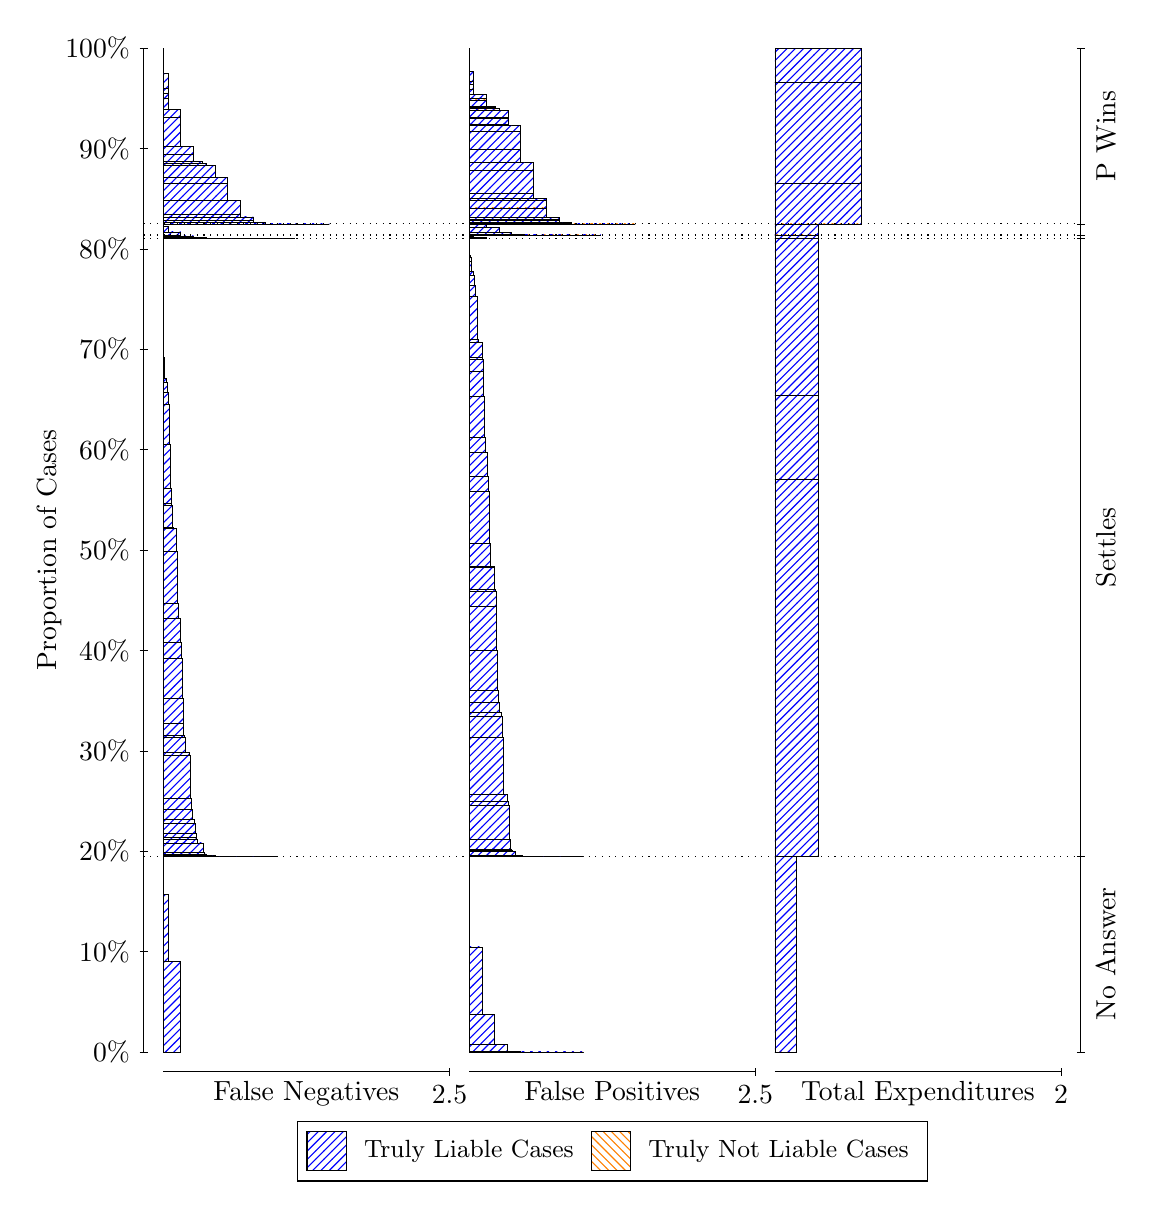
\begin{tikzpicture}
\draw[black, very thin] (1.5,1.75) -- (1.5,14.5);
\node[rotate=90, text=black, anchor=center] at (0.3, 8.125) {Proportion of Cases};
\draw[black, very thin] (1.45,1.75) -- (1.55,1.75);
\node[text=black, anchor=east] at (1.45, 1.75) {0\%};
\draw[black, very thin] (1.45,3.025) -- (1.55,3.025);
\node[text=black, anchor=east] at (1.45, 3.025) {10\%};
\draw[black, very thin] (1.45,4.3) -- (1.55,4.3);
\node[text=black, anchor=east] at (1.45, 4.3) {20\%};
\draw[black, very thin] (1.45,5.575) -- (1.55,5.575);
\node[text=black, anchor=east] at (1.45, 5.575) {30\%};
\draw[black, very thin] (1.45,6.85) -- (1.55,6.85);
\node[text=black, anchor=east] at (1.45, 6.85) {40\%};
\draw[black, very thin] (1.45,8.125) -- (1.55,8.125);
\node[text=black, anchor=east] at (1.45, 8.125) {50\%};
\draw[black, very thin] (1.45,9.4) -- (1.55,9.4);
\node[text=black, anchor=east] at (1.45, 9.4) {60\%};
\draw[black, very thin] (1.45,10.675) -- (1.55,10.675);
\node[text=black, anchor=east] at (1.45, 10.675) {70\%};
\draw[black, very thin] (1.45,11.95) -- (1.55,11.95);
\node[text=black, anchor=east] at (1.45, 11.95) {80\%};
\draw[black, very thin] (1.45,13.225) -- (1.55,13.225);
\node[text=black, anchor=east] at (1.45, 13.225) {90\%};
\draw[black, very thin] (1.45,14.5) -- (1.55,14.5);
\node[text=black, anchor=east] at (1.45, 14.5) {100\%};

\draw[black, very thin] (13.4,1.75) -- (13.4,14.5);
\draw[black, very thin] (13.35,1.75) -- (13.45,1.75);
\node[anchor=west] at (13.35, 1.75) {};
\draw[black, very thin] (13.35,4.2363) -- (13.45,4.2363);
\node[anchor=west] at (13.35, 4.2363) {};
\draw[black, very thin] (13.35,12.083) -- (13.45,12.083);
\node[anchor=west] at (13.35, 12.083) {};
\draw[black, very thin] (13.35,12.126) -- (13.45,12.126);
\node[anchor=west] at (13.35, 12.126) {};
\draw[black, very thin] (13.35,12.267) -- (13.45,12.267);
\node[anchor=west] at (13.35, 12.267) {};
\draw[black, very thin] (13.35,14.5) -- (13.45,14.5);
\node[anchor=west] at (13.35, 14.5) {};

\draw[black, very thin, pattern color=blue, pattern=north east lines] (1.75,1.75) rectangle (1.968,2.9018);
\draw[black, very thin, pattern color=blue, pattern=north east lines] (1.75,2.9018) rectangle (1.8065,3.7553);
\draw[black, very thin, pattern color=orange, pattern=north west lines] (1.75,3.7553) rectangle (1.75,3.7553);
\draw[black, very thin, pattern color=blue, pattern=north east lines] (1.75,3.7553) rectangle (1.75,4.2363);
\draw[black, very thin, pattern color=blue, pattern=north east lines] (1.75,4.2363) rectangle (3.2033,4.2363);
\draw[black, very thin, pattern color=blue, pattern=north east lines] (1.75,4.2363) rectangle (3.1307,4.2363);
\draw[black, very thin, pattern color=blue, pattern=north east lines] (1.75,4.2363) rectangle (3.058,4.2363);
\draw[black, very thin, pattern color=blue, pattern=north east lines] (1.75,4.2363) rectangle (3.0419,4.2363);
\draw[black, very thin, pattern color=blue, pattern=north east lines] (1.75,4.2363) rectangle (2.9853,4.2363);
\draw[black, very thin, pattern color=blue, pattern=north east lines] (1.75,4.2363) rectangle (2.9692,4.2363);
\draw[black, very thin, pattern color=blue, pattern=north east lines] (1.75,4.2363) rectangle (2.9127,4.2363);
\draw[black, very thin, pattern color=blue, pattern=north east lines] (1.75,4.2363) rectangle (2.8965,4.2363);
\draw[black, very thin, pattern color=blue, pattern=north east lines] (1.75,4.2363) rectangle (2.8804,4.2363);
\draw[black, very thin, pattern color=blue, pattern=north east lines] (1.75,4.2363) rectangle (2.84,4.2363);
\draw[black, very thin, pattern color=blue, pattern=north east lines] (1.75,4.2363) rectangle (2.8239,4.2363);
\draw[black, very thin, pattern color=blue, pattern=north east lines] (1.75,4.2363) rectangle (2.8077,4.2363);
\draw[black, very thin, pattern color=blue, pattern=north east lines] (1.75,4.2363) rectangle (2.7673,4.2363);
\draw[black, very thin, pattern color=blue, pattern=north east lines] (1.75,4.2363) rectangle (2.7512,4.2363);
\draw[black, very thin, pattern color=blue, pattern=north east lines] (1.75,4.2363) rectangle (2.735,4.2363);
\draw[black, very thin, pattern color=blue, pattern=north east lines] (1.75,4.2363) rectangle (2.7189,4.2363);
\draw[black, very thin, pattern color=blue, pattern=north east lines] (1.75,4.2363) rectangle (2.6947,4.2363);
\draw[black, very thin, pattern color=blue, pattern=north east lines] (1.75,4.2363) rectangle (2.6785,4.2363);
\draw[black, very thin, pattern color=blue, pattern=north east lines] (1.75,4.2363) rectangle (2.6624,4.2363);
\draw[black, very thin, pattern color=blue, pattern=north east lines] (1.75,4.2363) rectangle (2.6462,4.2363);
\draw[black, very thin, pattern color=blue, pattern=north east lines] (1.75,4.2363) rectangle (2.622,4.2363);
\draw[black, very thin, pattern color=blue, pattern=north east lines] (1.75,4.2363) rectangle (2.6059,4.2363);
\draw[black, very thin, pattern color=blue, pattern=north east lines] (1.75,4.2363) rectangle (2.5897,4.2363);
\draw[black, very thin, pattern color=blue, pattern=north east lines] (1.75,4.2363) rectangle (2.5736,4.2364);
\draw[black, very thin, pattern color=blue, pattern=north east lines] (1.75,4.2364) rectangle (2.5574,4.2364);
\draw[black, very thin, pattern color=blue, pattern=north east lines] (1.75,4.2364) rectangle (2.5332,4.2364);
\draw[black, very thin, pattern color=blue, pattern=north east lines] (1.75,4.2364) rectangle (2.517,4.2364);
\draw[black, very thin, pattern color=blue, pattern=north east lines] (1.75,4.2364) rectangle (2.5009,4.2364);
\draw[black, very thin, pattern color=blue, pattern=north east lines] (1.75,4.2364) rectangle (2.4847,4.2364);
\draw[black, very thin, pattern color=blue, pattern=north east lines] (1.75,4.2364) rectangle (2.4767,4.2365);
\draw[black, very thin, pattern color=blue, pattern=north east lines] (1.75,4.2365) rectangle (2.4605,4.2365);
\draw[black, very thin, pattern color=blue, pattern=north east lines] (1.75,4.2365) rectangle (2.4444,4.2366);
\draw[black, very thin, pattern color=blue, pattern=north east lines] (1.75,4.2366) rectangle (2.4282,4.2371);
\draw[black, very thin, pattern color=blue, pattern=north east lines] (1.75,4.2371) rectangle (2.4121,4.2428);
\draw[black, very thin, pattern color=blue, pattern=north east lines] (1.75,4.2428) rectangle (2.3959,4.2428);
\draw[black, very thin, pattern color=blue, pattern=north east lines] (1.75,4.2428) rectangle (2.3717,4.2428);
\draw[black, very thin, pattern color=blue, pattern=north east lines] (1.75,4.2428) rectangle (2.3556,4.2428);
\draw[black, very thin, pattern color=blue, pattern=north east lines] (1.75,4.2428) rectangle (2.3394,4.2429);
\draw[black, very thin, pattern color=blue, pattern=north east lines] (1.75,4.2429) rectangle (2.3313,4.2439);
\draw[black, very thin, pattern color=blue, pattern=north east lines] (1.75,4.2439) rectangle (2.3233,4.2463);
\draw[black, very thin, pattern color=blue, pattern=north east lines] (1.75,4.2463) rectangle (2.3152,4.2529);
\draw[black, very thin, pattern color=blue, pattern=north east lines] (1.75,4.2529) rectangle (2.299,4.2553);
\draw[black, very thin, pattern color=blue, pattern=north east lines] (1.75,4.2553) rectangle (2.2829,4.265);
\draw[black, very thin, pattern color=blue, pattern=north east lines] (1.75,4.265) rectangle (2.2667,4.2855);
\draw[black, very thin, pattern color=blue, pattern=north east lines] (1.75,4.2855) rectangle (2.2506,4.4038);
\draw[black, very thin, pattern color=blue, pattern=north east lines] (1.75,4.4038) rectangle (2.2344,4.4054);
\draw[black, very thin, pattern color=blue, pattern=north east lines] (1.75,4.4054) rectangle (2.2102,4.4054);
\draw[black, very thin, pattern color=blue, pattern=north east lines] (1.75,4.4054) rectangle (2.1941,4.4056);
\draw[black, very thin, pattern color=blue, pattern=north east lines] (1.75,4.4056) rectangle (2.186,4.4464);
\draw[black, very thin, pattern color=blue, pattern=north east lines] (1.75,4.4464) rectangle (2.1779,4.4494);
\draw[black, very thin, pattern color=blue, pattern=north east lines] (1.75,4.4494) rectangle (2.1699,4.473);
\draw[black, very thin, pattern color=blue, pattern=north east lines] (1.75,4.473) rectangle (2.1618,4.5301);
\draw[black, very thin, pattern color=blue, pattern=north east lines] (1.75,4.5301) rectangle (2.1537,4.6511);
\draw[black, very thin, pattern color=blue, pattern=north east lines] (1.75,4.6511) rectangle (2.1376,4.7013);
\draw[black, very thin, pattern color=blue, pattern=north east lines] (1.75,4.7013) rectangle (2.1214,4.8288);
\draw[black, very thin, pattern color=blue, pattern=north east lines] (1.75,4.8288) rectangle (2.1053,4.9764);
\draw[black, very thin, pattern color=blue, pattern=north east lines] (1.75,4.9764) rectangle (2.0891,5.5124);
\draw[black, very thin, pattern color=blue, pattern=north east lines] (1.75,5.5124) rectangle (2.073,5.5556);
\draw[black, very thin, pattern color=blue, pattern=north east lines] (1.75,5.5556) rectangle (2.0487,5.5556);
\draw[black, very thin, pattern color=blue, pattern=north east lines] (1.75,5.5556) rectangle (2.0326,5.558);
\draw[black, very thin, pattern color=blue, pattern=north east lines] (1.75,5.558) rectangle (2.0245,5.751);
\draw[black, very thin, pattern color=blue, pattern=north east lines] (1.75,5.751) rectangle (2.0164,5.7716);
\draw[black, very thin, pattern color=blue, pattern=north east lines] (1.75,5.7716) rectangle (2.0084,5.921);
\draw[black, very thin, pattern color=blue, pattern=north east lines] (1.75,5.921) rectangle (2.0003,6.2397);
\draw[black, very thin, pattern color=blue, pattern=north east lines] (1.75,6.2397) rectangle (1.9922,6.7561);
\draw[black, very thin, pattern color=blue, pattern=north east lines] (1.75,6.7561) rectangle (1.9761,6.9537);
\draw[black, very thin, pattern color=blue, pattern=north east lines] (1.75,6.9537) rectangle (1.9599,7.2572);
\draw[black, very thin, pattern color=blue, pattern=north east lines] (1.75,7.2572) rectangle (1.9438,7.4499);
\draw[black, very thin, pattern color=blue, pattern=north east lines] (1.75,7.4499) rectangle (1.9276,8.1082);
\draw[black, very thin, pattern color=blue, pattern=north east lines] (1.75,8.1082) rectangle (1.9115,8.4017);
\draw[black, very thin, pattern color=blue, pattern=north east lines] (1.75,8.4017) rectangle (1.8873,8.4018);
\draw[black, very thin, pattern color=blue, pattern=north east lines] (1.75,8.4018) rectangle (1.8711,8.4074);
\draw[black, very thin, pattern color=blue, pattern=north east lines] (1.75,8.4074) rectangle (1.863,8.6915);
\draw[black, very thin, pattern color=blue, pattern=north east lines] (1.75,8.6915) rectangle (1.855,8.7152);
\draw[black, very thin, pattern color=blue, pattern=north east lines] (1.75,8.7152) rectangle (1.8469,8.9078);
\draw[black, very thin, pattern color=blue, pattern=north east lines] (1.75,8.9078) rectangle (1.8388,9.462);
\draw[black, very thin, pattern color=blue, pattern=north east lines] (1.75,9.462) rectangle (1.8307,9.9782);
\draw[black, very thin, pattern color=blue, pattern=north east lines] (1.75,9.9782) rectangle (1.8146,10.128);
\draw[black, very thin, pattern color=blue, pattern=north east lines] (1.75,10.128) rectangle (1.7984,10.256);
\draw[black, very thin, pattern color=blue, pattern=north east lines] (1.75,10.256) rectangle (1.7823,10.305);
\draw[black, very thin, pattern color=blue, pattern=north east lines] (1.75,10.305) rectangle (1.7661,10.573);
\draw[black, very thin, pattern color=orange, pattern=north west lines] (1.75,10.573) rectangle (1.75,10.573);
\draw[black, very thin, pattern color=blue, pattern=north east lines] (1.75,10.573) rectangle (1.75,12.083);
\draw[black, very thin, pattern color=blue, pattern=north east lines] (1.75,12.083) rectangle (3.4213,12.083);
\draw[black, very thin, pattern color=blue, pattern=north east lines] (1.75,12.083) rectangle (3.2599,12.083);
\draw[black, very thin, pattern color=blue, pattern=north east lines] (1.75,12.083) rectangle (3.0984,12.083);
\draw[black, very thin, pattern color=blue, pattern=north east lines] (1.75,12.083) rectangle (2.9369,12.083);
\draw[black, very thin, pattern color=blue, pattern=north east lines] (1.75,12.083) rectangle (2.7754,12.083);
\draw[black, very thin, pattern color=blue, pattern=north east lines] (1.75,12.083) rectangle (2.6139,12.083);
\draw[black, very thin, pattern color=blue, pattern=north east lines] (1.75,12.083) rectangle (2.4524,12.084);
\draw[black, very thin, pattern color=blue, pattern=north east lines] (1.75,12.084) rectangle (2.291,12.093);
\draw[black, very thin, pattern color=blue, pattern=north east lines] (1.75,12.093) rectangle (2.1295,12.114);
\draw[black, very thin, pattern color=blue, pattern=north east lines] (1.75,12.114) rectangle (1.968,12.126);
\draw[black, very thin, pattern color=orange, pattern=north west lines] (1.75,12.126) rectangle (1.75,12.126);
\draw[black, very thin, pattern color=blue, pattern=north east lines] (1.75,12.126) rectangle (1.968,12.166);
\draw[black, very thin, pattern color=blue, pattern=north east lines] (1.75,12.166) rectangle (1.8065,12.232);
\draw[black, very thin, pattern color=orange, pattern=north west lines] (1.75,12.232) rectangle (1.75,12.232);
\draw[black, very thin, pattern color=blue, pattern=north east lines] (1.75,12.232) rectangle (1.75,12.267);
\draw[black, very thin, pattern color=blue, pattern=north east lines] (1.75,12.267) rectangle (3.8573,12.267);
\draw[black, very thin, pattern color=blue, pattern=north east lines] (1.75,12.267) rectangle (3.6959,12.267);
\draw[black, very thin, pattern color=blue, pattern=north east lines] (1.75,12.267) rectangle (3.5344,12.267);
\draw[black, very thin, pattern color=blue, pattern=north east lines] (1.75,12.267) rectangle (3.5344,12.267);
\draw[black, very thin, pattern color=blue, pattern=north east lines] (1.75,12.267) rectangle (3.3729,12.267);
\draw[black, very thin, pattern color=blue, pattern=north east lines] (1.75,12.267) rectangle (3.2114,12.268);
\draw[black, very thin, pattern color=blue, pattern=north east lines] (1.75,12.268) rectangle (3.0984,12.268);
\draw[black, very thin, pattern color=blue, pattern=north east lines] (1.75,12.268) rectangle (3.0499,12.282);
\draw[black, very thin, pattern color=blue, pattern=north east lines] (1.75,12.282) rectangle (2.9369,12.282);
\draw[black, very thin, pattern color=blue, pattern=north east lines] (1.75,12.282) rectangle (2.8884,12.309);
\draw[black, very thin, pattern color=blue, pattern=north east lines] (1.75,12.309) rectangle (2.8884,12.355);
\draw[black, very thin, pattern color=blue, pattern=north east lines] (1.75,12.355) rectangle (2.7754,12.355);
\draw[black, very thin, pattern color=blue, pattern=north east lines] (1.75,12.355) rectangle (2.7754,12.355);
\draw[black, very thin, pattern color=blue, pattern=north east lines] (1.75,12.355) rectangle (2.727,12.385);
\draw[black, very thin, pattern color=blue, pattern=north east lines] (1.75,12.385) rectangle (2.727,12.566);
\draw[black, very thin, pattern color=blue, pattern=north east lines] (1.75,12.566) rectangle (2.6139,12.566);
\draw[black, very thin, pattern color=blue, pattern=north east lines] (1.75,12.566) rectangle (2.5655,12.788);
\draw[black, very thin, pattern color=blue, pattern=north east lines] (1.75,12.788) rectangle (2.5655,12.853);
\draw[black, very thin, pattern color=blue, pattern=north east lines] (1.75,12.853) rectangle (2.4524,12.854);
\draw[black, very thin, pattern color=blue, pattern=north east lines] (1.75,12.854) rectangle (2.4524,12.854);
\draw[black, very thin, pattern color=blue, pattern=north east lines] (1.75,12.854) rectangle (2.404,13.007);
\draw[black, very thin, pattern color=blue, pattern=north east lines] (1.75,13.007) rectangle (2.291,13.031);
\draw[black, very thin, pattern color=blue, pattern=north east lines] (1.75,13.031) rectangle (2.2425,13.031);
\draw[black, very thin, pattern color=blue, pattern=north east lines] (1.75,13.031) rectangle (2.2425,13.059);
\draw[black, very thin, pattern color=blue, pattern=north east lines] (1.75,13.059) rectangle (2.2425,13.06);
\draw[black, very thin, pattern color=blue, pattern=north east lines] (1.75,13.06) rectangle (2.1295,13.151);
\draw[black, very thin, pattern color=blue, pattern=north east lines] (1.75,13.151) rectangle (2.1295,13.252);
\draw[black, very thin, pattern color=blue, pattern=north east lines] (1.75,13.252) rectangle (2.081,13.252);
\draw[black, very thin, pattern color=blue, pattern=north east lines] (1.75,13.252) rectangle (2.081,13.252);
\draw[black, very thin, pattern color=blue, pattern=north east lines] (1.75,13.252) rectangle (1.968,13.619);
\draw[black, very thin, pattern color=blue, pattern=north east lines] (1.75,13.619) rectangle (1.968,13.719);
\draw[black, very thin, pattern color=blue, pattern=north east lines] (1.75,13.719) rectangle (1.9196,13.719);
\draw[black, very thin, pattern color=blue, pattern=north east lines] (1.75,13.719) rectangle (1.9196,13.719);
\draw[black, very thin, pattern color=blue, pattern=north east lines] (1.75,13.719) rectangle (1.8065,13.858);
\draw[black, very thin, pattern color=blue, pattern=north east lines] (1.75,13.858) rectangle (1.8065,13.919);
\draw[black, very thin, pattern color=blue, pattern=north east lines] (1.75,13.919) rectangle (1.8065,13.985);
\draw[black, very thin, pattern color=blue, pattern=north east lines] (1.75,13.985) rectangle (1.8065,14.177);
\draw[black, very thin, pattern color=blue, pattern=north east lines] (1.75,14.177) rectangle (1.7581,14.177);
\draw[black, very thin, pattern color=blue, pattern=north east lines] (1.75,14.177) rectangle (1.7581,14.177);
\draw[black, very thin, pattern color=orange, pattern=north west lines] (1.75,14.177) rectangle (1.75,14.177);
\draw[black, very thin, pattern color=blue, pattern=north east lines] (1.75,14.177) rectangle (1.75,14.5);
\draw[black, very thin, pattern color=orange, pattern=north west lines] (5.6333,1.75) rectangle (7.0867,1.75);
\draw[black, very thin, pattern color=blue, pattern=north east lines] (5.6333,1.75) rectangle (7.0867,1.75);
\draw[black, very thin, pattern color=blue, pattern=north east lines] (5.6333,1.75) rectangle (6.9252,1.75);
\draw[black, very thin, pattern color=blue, pattern=north east lines] (5.6333,1.75) rectangle (6.7637,1.75);
\draw[black, very thin, pattern color=blue, pattern=north east lines] (5.6333,1.75) rectangle (6.6022,1.75);
\draw[black, very thin, pattern color=blue, pattern=north east lines] (5.6333,1.75) rectangle (6.4407,1.7503);
\draw[black, very thin, pattern color=blue, pattern=north east lines] (5.6333,1.7503) rectangle (6.2793,1.7582);
\draw[black, very thin, pattern color=blue, pattern=north east lines] (5.6333,1.7582) rectangle (6.1178,1.8431);
\draw[black, very thin, pattern color=blue, pattern=north east lines] (5.6333,1.8431) rectangle (5.9563,2.231);
\draw[black, very thin, pattern color=blue, pattern=north east lines] (5.6333,2.231) rectangle (5.7948,3.0845);
\draw[black, very thin, pattern color=blue, pattern=north east lines] (5.6333,3.0845) rectangle (5.6333,4.2363);
\draw[black, very thin, pattern color=orange, pattern=north west lines] (5.6333,4.2363) rectangle (7.0867,4.2363);
\draw[black, very thin, pattern color=blue, pattern=north east lines] (5.6333,4.2363) rectangle (7.0867,4.2363);
\draw[black, very thin, pattern color=orange, pattern=north west lines] (5.6333,4.2363) rectangle (6.9413,4.2363);
\draw[black, very thin, pattern color=blue, pattern=north east lines] (5.6333,4.2363) rectangle (6.9413,4.2363);
\draw[black, very thin, pattern color=blue, pattern=north east lines] (5.6333,4.2363) rectangle (6.9252,4.2363);
\draw[black, very thin, pattern color=orange, pattern=north west lines] (5.6333,4.2363) rectangle (6.796,4.2363);
\draw[black, very thin, pattern color=blue, pattern=north east lines] (5.6333,4.2363) rectangle (6.796,4.2363);
\draw[black, very thin, pattern color=blue, pattern=north east lines] (5.6333,4.2363) rectangle (6.7799,4.2363);
\draw[black, very thin, pattern color=blue, pattern=north east lines] (5.6333,4.2363) rectangle (6.7637,4.2363);
\draw[black, very thin, pattern color=orange, pattern=north west lines] (5.6333,4.2363) rectangle (6.6507,4.2363);
\draw[black, very thin, pattern color=blue, pattern=north east lines] (5.6333,4.2363) rectangle (6.6507,4.2363);
\draw[black, very thin, pattern color=blue, pattern=north east lines] (5.6333,4.2363) rectangle (6.6345,4.2363);
\draw[black, very thin, pattern color=blue, pattern=north east lines] (5.6333,4.2363) rectangle (6.6184,4.2363);
\draw[black, very thin, pattern color=blue, pattern=north east lines] (5.6333,4.2363) rectangle (6.6022,4.2363);
\draw[black, very thin, pattern color=orange, pattern=north west lines] (5.6333,4.2363) rectangle (6.578,4.2363);
\draw[black, very thin, pattern color=blue, pattern=north east lines] (5.6333,4.2363) rectangle (6.578,4.2363);
\draw[black, very thin, pattern color=orange, pattern=north west lines] (5.6333,4.2363) rectangle (6.5053,4.2363);
\draw[black, very thin, pattern color=blue, pattern=north east lines] (5.6333,4.2363) rectangle (6.5053,4.2363);
\draw[black, very thin, pattern color=blue, pattern=north east lines] (5.6333,4.2363) rectangle (6.4892,4.2363);
\draw[black, very thin, pattern color=blue, pattern=north east lines] (5.6333,4.2363) rectangle (6.473,4.2364);
\draw[black, very thin, pattern color=blue, pattern=north east lines] (5.6333,4.2364) rectangle (6.4569,4.2364);
\draw[black, very thin, pattern color=blue, pattern=north east lines] (5.6333,4.2364) rectangle (6.4407,4.2364);
\draw[black, very thin, pattern color=orange, pattern=north west lines] (5.6333,4.2364) rectangle (6.4327,4.2364);
\draw[black, very thin, pattern color=blue, pattern=north east lines] (5.6333,4.2364) rectangle (6.4327,4.2364);
\draw[black, very thin, pattern color=blue, pattern=north east lines] (5.6333,4.2364) rectangle (6.4165,4.2364);
\draw[black, very thin, pattern color=orange, pattern=north west lines] (5.6333,4.2364) rectangle (6.36,4.2364);
\draw[black, very thin, pattern color=blue, pattern=north east lines] (5.6333,4.2364) rectangle (6.36,4.2365);
\draw[black, very thin, pattern color=blue, pattern=north east lines] (5.6333,4.2365) rectangle (6.3439,4.2366);
\draw[black, very thin, pattern color=blue, pattern=north east lines] (5.6333,4.2366) rectangle (6.3277,4.2371);
\draw[black, very thin, pattern color=blue, pattern=north east lines] (5.6333,4.2371) rectangle (6.3116,4.2428);
\draw[black, very thin, pattern color=blue, pattern=north east lines] (5.6333,4.2428) rectangle (6.2954,4.2451);
\draw[black, very thin, pattern color=orange, pattern=north west lines] (5.6333,4.2451) rectangle (6.2873,4.2451);
\draw[black, very thin, pattern color=blue, pattern=north east lines] (5.6333,4.2451) rectangle (6.2873,4.2455);
\draw[black, very thin, pattern color=blue, pattern=north east lines] (5.6333,4.2455) rectangle (6.2793,4.2506);
\draw[black, very thin, pattern color=blue, pattern=north east lines] (5.6333,4.2506) rectangle (6.2712,4.2508);
\draw[black, very thin, pattern color=blue, pattern=north east lines] (5.6333,4.2508) rectangle (6.255,4.2508);
\draw[black, very thin, pattern color=orange, pattern=north west lines] (5.6333,4.2508) rectangle (6.2147,4.2508);
\draw[black, very thin, pattern color=blue, pattern=north east lines] (5.6333,4.2508) rectangle (6.2147,4.2967);
\draw[black, very thin, pattern color=blue, pattern=north east lines] (5.6333,4.2967) rectangle (6.1985,4.2993);
\draw[black, very thin, pattern color=blue, pattern=north east lines] (5.6333,4.2993) rectangle (6.1824,4.309);
\draw[black, very thin, pattern color=blue, pattern=north east lines] (5.6333,4.309) rectangle (6.1662,4.3298);
\draw[black, very thin, pattern color=blue, pattern=north east lines] (5.6333,4.3298) rectangle (6.1501,4.4492);
\draw[black, very thin, pattern color=orange, pattern=north west lines] (5.6333,4.4492) rectangle (6.142,4.4492);
\draw[black, very thin, pattern color=blue, pattern=north east lines] (5.6333,4.4492) rectangle (6.142,4.8795);
\draw[black, very thin, pattern color=blue, pattern=north east lines] (5.6333,4.8795) rectangle (6.1339,4.9278);
\draw[black, very thin, pattern color=blue, pattern=north east lines] (5.6333,4.9278) rectangle (6.1259,4.9332);
\draw[black, very thin, pattern color=blue, pattern=north east lines] (5.6333,4.9332) rectangle (6.1178,5.0226);
\draw[black, very thin, pattern color=blue, pattern=north east lines] (5.6333,5.0226) rectangle (6.1097,5.025);
\draw[black, very thin, pattern color=blue, pattern=north east lines] (5.6333,5.025) rectangle (6.0936,5.025);
\draw[black, very thin, pattern color=orange, pattern=north west lines] (5.6333,5.025) rectangle (6.0693,5.025);
\draw[black, very thin, pattern color=blue, pattern=north east lines] (5.6333,5.025) rectangle (6.0693,5.7462);
\draw[black, very thin, pattern color=blue, pattern=north east lines] (5.6333,5.7462) rectangle (6.0532,6.0144);
\draw[black, very thin, pattern color=blue, pattern=north east lines] (5.6333,6.0144) rectangle (6.037,6.0633);
\draw[black, very thin, pattern color=blue, pattern=north east lines] (5.6333,6.0633) rectangle (6.0209,6.1909);
\draw[black, very thin, pattern color=blue, pattern=north east lines] (5.6333,6.1909) rectangle (6.0047,6.3408);
\draw[black, very thin, pattern color=blue, pattern=north east lines] (5.6333,6.3408) rectangle (5.9886,6.857);
\draw[black, very thin, pattern color=blue, pattern=north east lines] (5.6333,6.857) rectangle (5.9805,7.4112);
\draw[black, very thin, pattern color=blue, pattern=north east lines] (5.6333,7.4112) rectangle (5.9724,7.6038);
\draw[black, very thin, pattern color=blue, pattern=north east lines] (5.6333,7.6038) rectangle (5.9644,7.6275);
\draw[black, very thin, pattern color=blue, pattern=north east lines] (5.6333,7.6275) rectangle (5.9563,7.9116);
\draw[black, very thin, pattern color=blue, pattern=north east lines] (5.6333,7.9116) rectangle (5.9482,7.9172);
\draw[black, very thin, pattern color=blue, pattern=north east lines] (5.6333,7.9172) rectangle (5.9321,7.9173);
\draw[black, very thin, pattern color=blue, pattern=north east lines] (5.6333,7.9173) rectangle (5.9079,8.2108);
\draw[black, very thin, pattern color=blue, pattern=north east lines] (5.6333,8.2108) rectangle (5.8917,8.8691);
\draw[black, very thin, pattern color=blue, pattern=north east lines] (5.6333,8.8691) rectangle (5.8756,9.0618);
\draw[black, very thin, pattern color=blue, pattern=north east lines] (5.6333,9.0618) rectangle (5.8594,9.3653);
\draw[black, very thin, pattern color=blue, pattern=north east lines] (5.6333,9.3653) rectangle (5.8433,9.5629);
\draw[black, very thin, pattern color=blue, pattern=north east lines] (5.6333,9.5629) rectangle (5.8271,10.079);
\draw[black, very thin, pattern color=blue, pattern=north east lines] (5.6333,10.079) rectangle (5.819,10.398);
\draw[black, very thin, pattern color=blue, pattern=north east lines] (5.6333,10.398) rectangle (5.811,10.547);
\draw[black, very thin, pattern color=blue, pattern=north east lines] (5.6333,10.547) rectangle (5.8029,10.568);
\draw[black, very thin, pattern color=blue, pattern=north east lines] (5.6333,10.568) rectangle (5.7948,10.761);
\draw[black, very thin, pattern color=blue, pattern=north east lines] (5.6333,10.761) rectangle (5.7867,10.763);
\draw[black, very thin, pattern color=blue, pattern=north east lines] (5.6333,10.763) rectangle (5.7706,10.763);
\draw[black, very thin, pattern color=blue, pattern=north east lines] (5.6333,10.763) rectangle (5.7464,10.807);
\draw[black, very thin, pattern color=blue, pattern=north east lines] (5.6333,10.807) rectangle (5.7302,11.343);
\draw[black, very thin, pattern color=blue, pattern=north east lines] (5.6333,11.343) rectangle (5.7141,11.49);
\draw[black, very thin, pattern color=blue, pattern=north east lines] (5.6333,11.49) rectangle (5.6979,11.618);
\draw[black, very thin, pattern color=blue, pattern=north east lines] (5.6333,11.618) rectangle (5.6818,11.668);
\draw[black, very thin, pattern color=blue, pattern=north east lines] (5.6333,11.668) rectangle (5.6656,11.789);
\draw[black, very thin, pattern color=blue, pattern=north east lines] (5.6333,11.789) rectangle (5.6576,11.846);
\draw[black, very thin, pattern color=blue, pattern=north east lines] (5.6333,11.846) rectangle (5.6495,11.87);
\draw[black, very thin, pattern color=blue, pattern=north east lines] (5.6333,11.87) rectangle (5.6414,11.873);
\draw[black, very thin, pattern color=blue, pattern=north east lines] (5.6333,11.873) rectangle (5.6333,12.083);
\draw[black, very thin, pattern color=orange, pattern=north west lines] (5.6333,12.083) rectangle (5.8513,12.083);
\draw[black, very thin, pattern color=blue, pattern=north east lines] (5.6333,12.083) rectangle (5.8513,12.095);
\draw[black, very thin, pattern color=blue, pattern=north east lines] (5.6333,12.095) rectangle (5.6899,12.115);
\draw[black, very thin, pattern color=blue, pattern=north east lines] (5.6333,12.115) rectangle (5.6333,12.126);
\draw[black, very thin, pattern color=orange, pattern=north west lines] (5.6333,12.126) rectangle (7.3047,12.126);
\draw[black, very thin, pattern color=blue, pattern=north east lines] (5.6333,12.126) rectangle (7.3047,12.126);
\draw[black, very thin, pattern color=blue, pattern=north east lines] (5.6333,12.126) rectangle (7.1432,12.126);
\draw[black, very thin, pattern color=blue, pattern=north east lines] (5.6333,12.126) rectangle (6.9817,12.126);
\draw[black, very thin, pattern color=blue, pattern=north east lines] (5.6333,12.126) rectangle (6.8202,12.126);
\draw[black, very thin, pattern color=blue, pattern=north east lines] (5.6333,12.126) rectangle (6.6587,12.126);
\draw[black, very thin, pattern color=blue, pattern=north east lines] (5.6333,12.126) rectangle (6.4973,12.126);
\draw[black, very thin, pattern color=blue, pattern=north east lines] (5.6333,12.126) rectangle (6.3358,12.13);
\draw[black, very thin, pattern color=blue, pattern=north east lines] (5.6333,12.13) rectangle (6.1743,12.161);
\draw[black, very thin, pattern color=blue, pattern=north east lines] (5.6333,12.161) rectangle (6.0128,12.226);
\draw[black, very thin, pattern color=blue, pattern=north east lines] (5.6333,12.226) rectangle (5.8513,12.267);
\draw[black, very thin, pattern color=orange, pattern=north west lines] (5.6333,12.267) rectangle (7.7407,12.267);
\draw[black, very thin, pattern color=blue, pattern=north east lines] (5.6333,12.267) rectangle (7.7407,12.267);
\draw[black, very thin, pattern color=orange, pattern=north west lines] (5.6333,12.267) rectangle (7.5792,12.267);
\draw[black, very thin, pattern color=blue, pattern=north east lines] (5.6333,12.267) rectangle (7.5792,12.267);
\draw[black, very thin, pattern color=orange, pattern=north west lines] (5.6333,12.267) rectangle (7.4177,12.267);
\draw[black, very thin, pattern color=blue, pattern=north east lines] (5.6333,12.267) rectangle (7.4177,12.267);
\draw[black, very thin, pattern color=blue, pattern=north east lines] (5.6333,12.267) rectangle (7.4177,12.267);
\draw[black, very thin, pattern color=orange, pattern=north west lines] (5.6333,12.267) rectangle (7.2562,12.267);
\draw[black, very thin, pattern color=blue, pattern=north east lines] (5.6333,12.267) rectangle (7.2562,12.267);
\draw[black, very thin, pattern color=orange, pattern=north west lines] (5.6333,12.267) rectangle (7.0947,12.267);
\draw[black, very thin, pattern color=blue, pattern=north east lines] (5.6333,12.267) rectangle (7.0947,12.268);
\draw[black, very thin, pattern color=orange, pattern=north west lines] (5.6333,12.268) rectangle (6.9817,12.268);
\draw[black, very thin, pattern color=blue, pattern=north east lines] (5.6333,12.268) rectangle (6.9817,12.268);
\draw[black, very thin, pattern color=blue, pattern=north east lines] (5.6333,12.268) rectangle (6.9333,12.271);
\draw[black, very thin, pattern color=blue, pattern=north east lines] (5.6333,12.271) rectangle (6.9333,12.272);
\draw[black, very thin, pattern color=orange, pattern=north west lines] (5.6333,12.272) rectangle (6.9333,12.272);
\draw[black, very thin, pattern color=blue, pattern=north east lines] (5.6333,12.272) rectangle (6.9333,12.281);
\draw[black, very thin, pattern color=orange, pattern=north west lines] (5.6333,12.281) rectangle (6.8202,12.281);
\draw[black, very thin, pattern color=blue, pattern=north east lines] (5.6333,12.281) rectangle (6.8202,12.281);
\draw[black, very thin, pattern color=blue, pattern=north east lines] (5.6333,12.281) rectangle (6.7718,12.309);
\draw[black, very thin, pattern color=blue, pattern=north east lines] (5.6333,12.309) rectangle (6.7718,12.328);
\draw[black, very thin, pattern color=orange, pattern=north west lines] (5.6333,12.328) rectangle (6.7718,12.328);
\draw[black, very thin, pattern color=blue, pattern=north east lines] (5.6333,12.328) rectangle (6.7718,12.351);
\draw[black, very thin, pattern color=orange, pattern=north west lines] (5.6333,12.351) rectangle (6.6587,12.351);
\draw[black, very thin, pattern color=blue, pattern=north east lines] (5.6333,12.351) rectangle (6.6587,12.351);
\draw[black, very thin, pattern color=blue, pattern=north east lines] (5.6333,12.351) rectangle (6.6587,12.351);
\draw[black, very thin, pattern color=blue, pattern=north east lines] (5.6333,12.351) rectangle (6.6103,12.471);
\draw[black, very thin, pattern color=orange, pattern=north west lines] (5.6333,12.471) rectangle (6.6103,12.471);
\draw[black, very thin, pattern color=blue, pattern=north east lines] (5.6333,12.471) rectangle (6.6103,12.572);
\draw[black, very thin, pattern color=blue, pattern=north east lines] (5.6333,12.572) rectangle (6.6103,12.589);
\draw[black, very thin, pattern color=blue, pattern=north east lines] (5.6333,12.589) rectangle (6.4973,12.589);
\draw[black, very thin, pattern color=orange, pattern=north west lines] (5.6333,12.589) rectangle (6.4973,12.589);
\draw[black, very thin, pattern color=blue, pattern=north east lines] (5.6333,12.589) rectangle (6.4973,12.589);
\draw[black, very thin, pattern color=blue, pattern=north east lines] (5.6333,12.589) rectangle (6.4488,12.658);
\draw[black, very thin, pattern color=blue, pattern=north east lines] (5.6333,12.658) rectangle (6.4488,12.946);
\draw[black, very thin, pattern color=blue, pattern=north east lines] (5.6333,12.946) rectangle (6.4488,13.048);
\draw[black, very thin, pattern color=blue, pattern=north east lines] (5.6333,13.048) rectangle (6.3358,13.048);
\draw[black, very thin, pattern color=blue, pattern=north east lines] (5.6333,13.048) rectangle (6.3358,13.048);
\draw[black, very thin, pattern color=orange, pattern=north west lines] (5.6333,13.048) rectangle (6.3358,13.048);
\draw[black, very thin, pattern color=blue, pattern=north east lines] (5.6333,13.048) rectangle (6.3358,13.048);
\draw[black, very thin, pattern color=blue, pattern=north east lines] (5.6333,13.048) rectangle (6.2873,13.209);
\draw[black, very thin, pattern color=blue, pattern=north east lines] (5.6333,13.209) rectangle (6.2873,13.439);
\draw[black, very thin, pattern color=blue, pattern=north east lines] (5.6333,13.439) rectangle (6.2873,13.515);
\draw[black, very thin, pattern color=blue, pattern=north east lines] (5.6333,13.515) rectangle (6.1743,13.515);
\draw[black, very thin, pattern color=orange, pattern=north west lines] (5.6333,13.515) rectangle (6.1743,13.515);
\draw[black, very thin, pattern color=blue, pattern=north east lines] (5.6333,13.515) rectangle (6.1743,13.515);
\draw[black, very thin, pattern color=blue, pattern=north east lines] (5.6333,13.515) rectangle (6.1743,13.515);
\draw[black, very thin, pattern color=blue, pattern=north east lines] (5.6333,13.515) rectangle (6.1259,13.536);
\draw[black, very thin, pattern color=blue, pattern=north east lines] (5.6333,13.536) rectangle (6.1259,13.614);
\draw[black, very thin, pattern color=blue, pattern=north east lines] (5.6333,13.614) rectangle (6.1259,13.619);
\draw[black, very thin, pattern color=blue, pattern=north east lines] (5.6333,13.619) rectangle (6.1259,13.707);
\draw[black, very thin, pattern color=blue, pattern=north east lines] (5.6333,13.707) rectangle (6.0128,13.708);
\draw[black, very thin, pattern color=blue, pattern=north east lines] (5.6333,13.708) rectangle (6.0128,13.713);
\draw[black, very thin, pattern color=orange, pattern=north west lines] (5.6333,13.713) rectangle (6.0128,13.713);
\draw[black, very thin, pattern color=blue, pattern=north east lines] (5.6333,13.713) rectangle (6.0128,13.735);
\draw[black, very thin, pattern color=blue, pattern=north east lines] (5.6333,13.735) rectangle (5.9644,13.748);
\draw[black, very thin, pattern color=blue, pattern=north east lines] (5.6333,13.748) rectangle (5.9644,13.75);
\draw[black, very thin, pattern color=blue, pattern=north east lines] (5.6333,13.75) rectangle (5.9644,13.759);
\draw[black, very thin, pattern color=blue, pattern=north east lines] (5.6333,13.759) rectangle (5.8513,13.84);
\draw[black, very thin, pattern color=orange, pattern=north west lines] (5.6333,13.84) rectangle (5.8513,13.84);
\draw[black, very thin, pattern color=blue, pattern=north east lines] (5.6333,13.84) rectangle (5.8513,13.866);
\draw[black, very thin, pattern color=blue, pattern=north east lines] (5.6333,13.866) rectangle (5.8513,13.912);
\draw[black, very thin, pattern color=blue, pattern=north east lines] (5.6333,13.912) rectangle (5.8029,13.913);
\draw[black, very thin, pattern color=blue, pattern=north east lines] (5.6333,13.913) rectangle (5.8029,13.913);
\draw[black, very thin, pattern color=blue, pattern=north east lines] (5.6333,13.913) rectangle (5.6899,13.978);
\draw[black, very thin, pattern color=blue, pattern=north east lines] (5.6333,13.978) rectangle (5.6899,14.039);
\draw[black, very thin, pattern color=blue, pattern=north east lines] (5.6333,14.039) rectangle (5.6899,14.072);
\draw[black, very thin, pattern color=blue, pattern=north east lines] (5.6333,14.072) rectangle (5.6899,14.201);
\draw[black, very thin, pattern color=blue, pattern=north east lines] (5.6333,14.201) rectangle (5.6414,14.201);
\draw[black, very thin, pattern color=blue, pattern=north east lines] (5.6333,14.201) rectangle (5.6414,14.201);
\draw[black, very thin, pattern color=blue, pattern=north east lines] (5.6333,14.201) rectangle (5.6333,14.5);
\draw[black, very thin, pattern color=orange, pattern=north west lines] (9.5167,1.75) rectangle (9.7892,1.75);
\draw[black, very thin, pattern color=blue, pattern=north east lines] (9.5167,1.75) rectangle (9.7892,4.2363);
\draw[black, very thin, pattern color=orange, pattern=north west lines] (9.5167,4.2363) rectangle (10.062,4.2363);
\draw[black, very thin, pattern color=blue, pattern=north east lines] (9.5167,4.2363) rectangle (10.062,9.0291);
\draw[black, very thin, pattern color=orange, pattern=north west lines] (9.5167,9.0291) rectangle (10.062,9.0291);
\draw[black, very thin, pattern color=blue, pattern=north east lines] (9.5167,9.0291) rectangle (10.062,10.089);
\draw[black, very thin, pattern color=orange, pattern=north west lines] (9.5167,10.089) rectangle (10.062,10.089);
\draw[black, very thin, pattern color=blue, pattern=north east lines] (9.5167,10.089) rectangle (10.062,12.083);
\draw[black, very thin, pattern color=orange, pattern=north west lines] (9.5167,12.083) rectangle (10.062,12.083);
\draw[black, very thin, pattern color=blue, pattern=north east lines] (9.5167,12.083) rectangle (10.062,12.126);
\draw[black, very thin, pattern color=orange, pattern=north west lines] (9.5167,12.126) rectangle (10.062,12.126);
\draw[black, very thin, pattern color=blue, pattern=north east lines] (9.5167,12.126) rectangle (10.062,12.267);
\draw[black, very thin, pattern color=orange, pattern=north west lines] (9.5167,12.267) rectangle (10.607,12.267);
\draw[black, very thin, pattern color=blue, pattern=north east lines] (9.5167,12.267) rectangle (10.607,12.784);
\draw[black, very thin, pattern color=orange, pattern=north west lines] (9.5167,12.784) rectangle (10.607,12.784);
\draw[black, very thin, pattern color=blue, pattern=north east lines] (9.5167,12.784) rectangle (10.607,14.068);
\draw[black, very thin, pattern color=orange, pattern=north west lines] (9.5167,14.068) rectangle (10.607,14.068);
\draw[black, very thin, pattern color=blue, pattern=north east lines] (9.5167,14.068) rectangle (10.607,14.5);
\draw[black, dotted] (1.5,4.2363) -- (13.4,4.2363);
\draw[black, dotted] (1.5,12.083) -- (13.4,12.083);
\draw[black, dotted] (1.5,12.126) -- (13.4,12.126);
\draw[black, dotted] (1.5,12.267) -- (13.4,12.267);
\draw[black, very thin] (1.75,1.5) -- (5.3833,1.5);
\node[text=black, anchor=north] at (3.5667, 1.5) {False Negatives};
\draw[black, very thin] (5.3833,1.45) -- (5.3833,1.55);
\node[text=black, anchor=north] at (5.3833, 1.45) {2.5};

\draw[black, very thin] (5.6333,1.5) -- (9.2667,1.5);
\node[text=black, anchor=north] at (7.45, 1.5) {False Positives};
\draw[black, very thin] (9.2667,1.45) -- (9.2667,1.55);
\node[text=black, anchor=north] at (9.2667, 1.45) {2.5};

\draw[black, very thin] (9.5167,1.5) -- (13.15,1.5);
\node[text=black, anchor=north] at (11.333, 1.5) {Total Expenditures};
\draw[black, very thin] (13.15,1.45) -- (13.15,1.55);
\node[text=black, anchor=north] at (13.15, 1.45) {2};

\node[text=black, centered, rotate=90] at (13.72, 2.9932) {No Answer};
\node[text=black, centered, rotate=90] at (13.72, 8.1595) {Settles};


\node[text=black, centered, rotate=90] at (13.72, 13.383) {P Wins};

\draw (7.449999999999999,1.5) node[draw=none] (baseCoordinate) {};
\begin{scope}[align=center]
        \matrix[scale=0.5, draw=black, below=0.5cm of baseCoordinate, nodes={draw}, column sep=0.1cm]{
            \node[rectangle, draw, minimum width=0.5cm, minimum height=0.5cm, pattern color=blue, pattern=north east lines] {}; &
            \node[draw=none, font=\small, text=black] (B) {Truly Liable Cases}; &
            \node[rectangle, draw, minimum width=0.5cm, minimum height=0.5cm, pattern color=orange, pattern=north west lines] {}; &
            \node[draw=none, font=\small, text=black] (B) {Truly Not Liable Cases}; \\
            };
\end{scope}

\end{tikzpicture}
\end{document}